\chapter{Related Work}
\label{cha:relatedwork}
Dieses Kapitel betrachtet drei wissenschaftliche Publikationen, die dieser Arbeit nahe stehen. Dabei handelt es sich um die Arbeiten \emph{A Deployable Routing System for Nanonetworks} von Liaskos et al., \emph{CORONA: A Coordinate and Routing system for Nanonetworks} von Tsioliaridou et al. und \emph{Hop Count Routing: A Routing Algorithm for Resource Constrained, Identity-Free Medical Nanonetworks} von Büther et al., die alle verschiedene Ansätze für Routing und Koordination von Nanonetzwerken liefern \cite{buether2018hop, tsioliaridou2015corona, liaskos2016routing}. Alle drei Arbeiten wurden kurz im Kapitel~\ref{cha:grundlagen} vorgestellt. In den folgenden Sektionen sollen diese Arbeiten jedoch noch näher betrachtet und vorgestellt werden, da sie von besonderem Interesse für diese Arbeit sind.

\section{Hop Count Routing: A Routing Alogrithm for Resource Constraint, Identity-Free Medical Nanonetworks}

%\section{Hop Count Routing}

Die zuerst betrachtete Arbeit wurde im Jahr 2018 von Florian Büther, Immo Traupe und Sebastian Ebers verfasst \cite{buether2018hop}. Sie wurde mit besonderem Augenmerk auf \emph{In-Body-Networks} (IBN) und \emph{Body-Area-Networks} (BAN) verfasst. Die Nanogeräte in einem solchen Netzwerk unterliegen aufgrund des medizinischen Anwendungsfalls einigen Annahmen. So wird angenommen, dass ein Nanogerät in einem solchen Netzwerk verschiedene Komponenten besitzt: Eine Energieversorgung, eine einfache Recheneinheit, Sensoren und Aktuatoren, die eine aktive Kommunikation über elektromagnetische Terahertzwellen ermöglichen.  Da sich diese Nanogeräte jedoch im menschlichen Körper befinden, können Terahertzwellen nur auf einer Entfernung von ungefähr zwei Millimetern zuverlässig erkannt werden. Aus diesem Grund müssen die Nanogeräte ein Netzwerk aus vielen identischen Einheiten bilden. So kann der Hop-Count genutzt werden, um ein System zu entwickeln, das sowohl in Bezug auf Energie als auch Berechnung effizient ist.
Das in dieser Arbeit vorgestellte Hop-Count-Routing ist Gateway-orientiert. Es gibt ein Gateway auf Mikroebene, das Daten in das Nanonetzwerk sendet oder empfängt. Dabei gibt es zwei Phasen, die zum Routing benötigt werden: die Propagierungsphase und die Routingphase. 

In der Propagierungsphase erhalten alle Nanoknoten im System zu Beginn den Hop-Count $\infty$. Das Gateway sendet eine Nachricht in das Netzwerk mit dem eigenen Hop-Count $0$. Alle Empfängerknoten mit Hop-Count $n_r$ und einer beliebigen Nachricht mit Hop-Count $n_s$ verfahren in der Propagierungsphase wie folgt: Wenn $n_r > n_s + 1$ gilt, dann aktualisiere den eigenen Hop-Count auf $n_s + 1$ und sende den aktualisierten Wert in einer neuen Nachricht im Broadcast weiter. Wenn $n_r \leq n_s + 1$ gilt, dann mache nichts weiter. Da zu Beginn alle Knoten den Hop-Count $\infty$ besitzen, wird jeder Knoten im Netzwerk mindestens einmal aktualisiert und sendet den Hop-Count weiter. Das Ergebnis einer solchen Propagierungsphase ist in Abbildung~\ref{fig:hop-count} zu erkennen. Haben so alle Knoten den minimalen Hop-Count zum Gateway berechnet, so kann die Routingphase durchgeführt werden. 

\begin{figure}
    \centering
    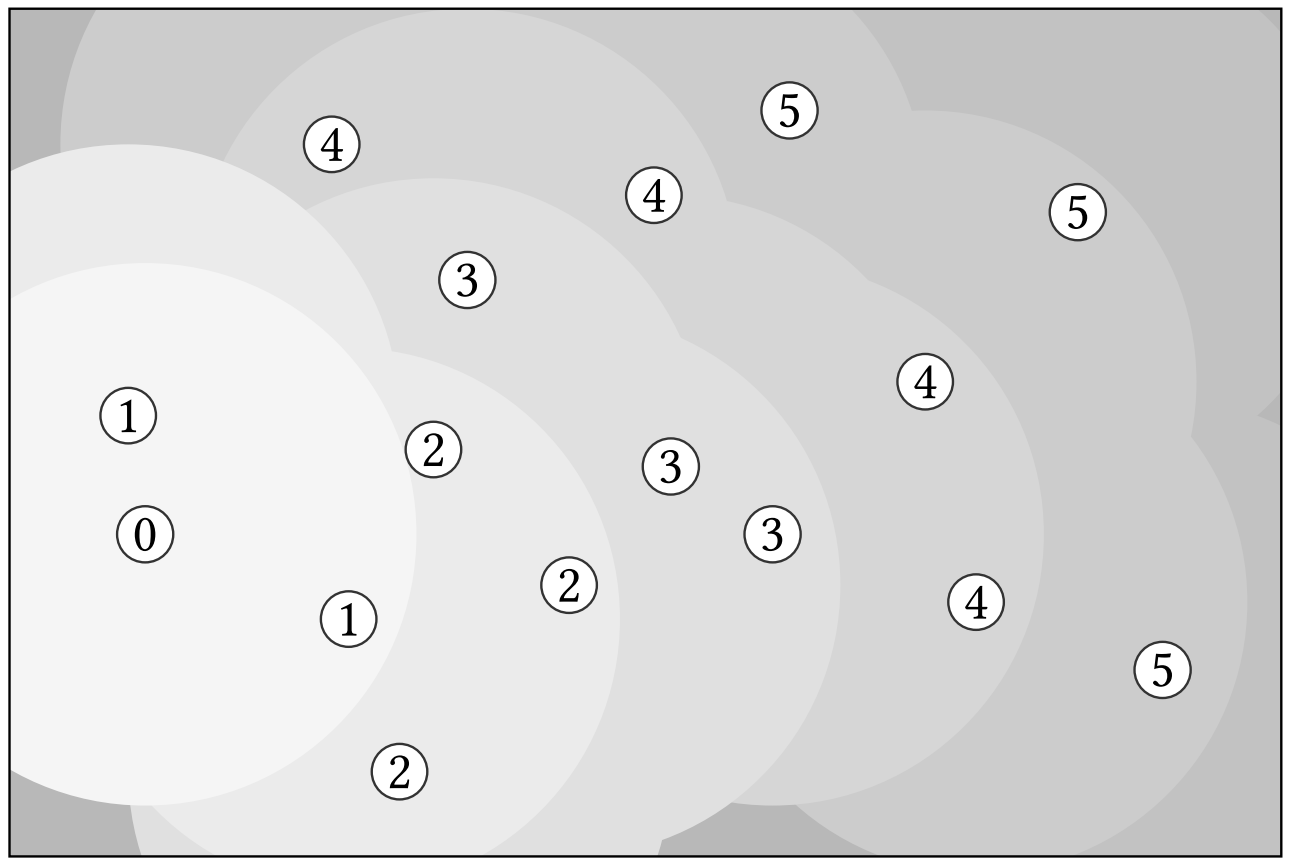
\includegraphics[width=0.65\textwidth]{images/Hop-Count.png}
    \caption[Grafische Darstellung eines gatewayorientierten Hop-Counts]{Grafische Darstellung eines gatewayorientierten Hop-Counts nach der Propagierungsphase. Dabei wird die Reichweite einzelner Knoten durch verschiedene Helligkeitsstufen dargestellt. Die Zahl, mit welcher ein Knoten bezeichnet ist, stellt dabei die Anzahl der Hops zwischen Gateway und Knoten dar.}
    \label{fig:hop-count}
\end{figure}

Während der Routingphase erfolgt eine Unterscheidung zwischen zwei Arten von Nachrichten. Die erste Art umfasst Nachrichten, die von einem Nanoknoten zum Gateway gesendet werden. In diesem Fall muss die Nachricht per Broadcast mit dem aktuellen Hop-Count versehen werden. Alle Knoten überprüfen, wenn sie eine Nachricht empfangen, ob ihr eigener Hop-Count kleiner ist als der in der Nachricht angegebene Hop-Count. Wenn dies der Fall ist, leitet der Knoten die Nachricht mit seinem eigenen Hop-Count weiter. Andernfalls wird nichts weiter unternommen. Die zweite Art von Nachrichten besteht aus Nachrichten, die vom Gateway an einen spezifischen Nanoknoten gesendet werden. In diesem Fall erfolgt eine ähnliche Überprüfung, bei der abgefragt wird, ob der eigene Hop-Count größer ist als der empfangene Hop-Count.

Bei diesem Hop-Count-Routing werden eine große Anzahl von Nanoknoten in jeder Übertragung beteiligt. Eine Optimierung, die diese Überlastung des Netzes verhindern soll, ist die \emph{destruktive Erfassung}. Dabei wird durch Änderung des Hop-Counts sichergestellt, dass alle Knoten nur einmal die Nachricht übertragen. Das führt dazu, dass Nachrichtenübertragungen in einem solchen Netzwerk nur noch sequentiell abläuft und nach einer Nachricht eine neue Propagierungsphase notwendig ist. Dieser Ansatz kann auch dazu führen, dass Übertragungen von Nanoknoten zum Gateway nicht ankommen, da die Knoten um das Gateway herum durch eine Nachricht zuvor genutzt wurden. Eine mögliche Lösung dieses Problems wäre, mehrere Gateways in einem System zu nutzen und alle Knoten den Hop-Count zu jedem Gateway speichern zu lassen. Hier würden aber erhöhte Speicherkosten und weitere Flags in der Nachricht anfallen. 

Bei der Auswertung des naiven und destruktiven Ansatzes für das Hop-Count-Routing kommen die Autoren der Arbeit zu dem Schluss, dass beide Ansätze schnell sind. Auch wenn der destruktive Ansatz eine geringere Nachrichtenmenge benötigt, ist der naive Ansatz ebenfalls einfach und schnell. Der worst-case von $\mathcal{O}(n^2)$ ist in realistischen Implementierungen unwahrscheinlich. Die Laufzeit des Algorithmus ist in der Simulation gut, jedoch wurden einige Annahmen gemacht, die in der Praxis erneut betrachtet werden müssen. In den Simulationen wird angenommen, dass die Nanoknoten statisch immer an derselben Stelle liegen. In einem medizinischen Anwendungsfall, in welchem dieses Netzwerk im menschlichen Körper liegt, ist dies wahrscheinlich nicht der Fall. Außerdem wird beim Modell des Nanoknotens nicht betrachtet, wie viel Zeit die Übertragung und Berechnung im Knoten selbst benötigt.

Abschließend ist zu dieser Arbeit zu sagen, dass ein interessanter und schneller Hop-Count-Routing Algorithmus geliefert wird, der in Hinsicht auf medizinische Body-Area-Networks entwickelt wird. Da einige vereinfachte Annahmen im Modell enthalten sind, muss sich ein solcher Ansatz jedoch noch in einem praxisnäheren Experiment bewähren.

Da sich die Arbeit auf Routing mit Terahertzwellen fokussiert, lässt sich der Algorithmus nicht auf DNA-Tiles und Self-Assemblies übertragen. Das Prinzip eines Body-Area-Networks, das die komplexeren Aufgaben des Netzwerkes übernimmt, ist jedoch interessant in Hinsicht auf die in dieser Masterarbeit betrachteten Nanonetzwerke. Ein Netzwerk auf Mikroebene, das über Gateways Tiles in ein Nanonetzwerk sendet und so mit Nanogeräten und Nanorobotern kommuniziert, stellt ein realistisches Anwendungsbeispiel für DNA-basierte Nanonetzwerke dar.

\section{CORONA: A Coordinate and Routing system for Nanonetworks}

In dieser Arbeit wird das koordinatenbasierte Routing-System CORONA vorgestellt. Das aus dem Jahr 2015 stammende Paper wurde von Ageliki Tsioliaridou, Christos Liaskos, Sotiris Ioannidis und Andreas Pitsillides verfasst \cite{tsioliaridou2015corona}. Das Routing-System basiert auf zwei Annahmen: Das Nanonetzwerk, in welchem es eingesetzt wird, ist vertrauenswürdig und benötigt keine weiteren Sicherheitsmechanismen und die Knoten befinden sich im zweidimensionalen Raum. Auch wird in dieser Arbeit davon ausgegangen, dass ein Knoten in diesem Netzwerk eine Nanomaschine ist, die aus einer Energiequelle, einem Speicher, einer Antenne und einer Recheneinheit besteht. Dabei können alle Knoten autonom einfache Operationen ausführen und über kurze Strecken kommunizieren. 

\begin{figure}
    \centering
    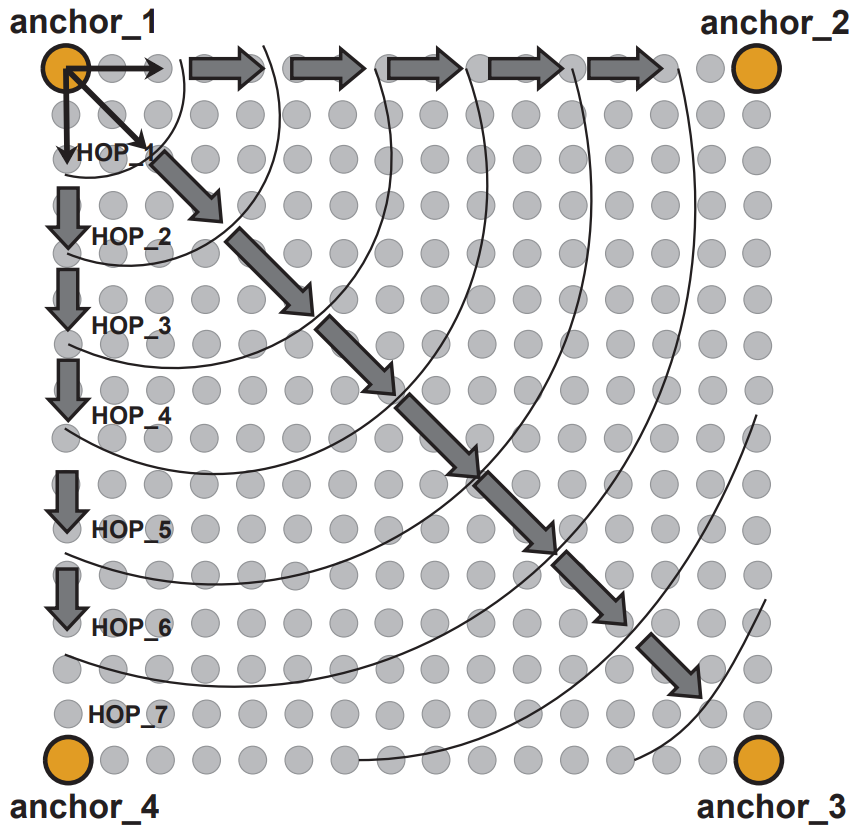
\includegraphics[width=0.5\textwidth]{images/Corona.png}
    \caption[CORONA Ankerpunkte Verbildlichung]{Darstellung eines rechteckigen Gebiets in einem Nanonetzwerk. Die vier Eckpunkte des Gebiets bilden die Ankerpunkte und definieren über die Entfernung zu den einzelnen Knoten über Hops die eindeutigen Positionen jedes Nanoknotens im Gebiet. Abbildung aus der Arbeit von Tsioliaridou et al. \cite{tsioliaridou2015corona}}
    \label{fig:corona}
\end{figure}

Das System basiert auf der Idee, dass Nanonetzwerke in den meisten Anwendungsfällen vorwiegend datenzentriert funktionieren. Ein Ansatz aus einer früheren Arbeit, der einen wiederholten Broadcast aller Nachrichten durchführt, soll in dieser Arbeit durch ein Unicast-basiertes System ersetzt werden \cite{liaskos2015flood}. Die Arbeit legt den Fokus bei Nanomaschinen auf \emph{Software-Defined Metamaterials} (SDM), einer neuen Klasse von künstlichen Materialien mit programmierbaren elektromagnetischen Eigenschaften \cite{liaskos2015sdm}. Mit diesen Grundlagen werden in einem rechteckigen Gebiet Nanoknoten platziert. Die vier Ecken des Rechtecks werden dabei als Ankerpunkte definiert. Auf Basis von Standard-Triangulation können so allen Nanoknoten in diesem Gebiet eindeutige Koordinaten gegeben werden, indem die Entfernung über Hops zwischen dem Knoten und den Ankerpunkten definiert wird. Dieser Vorgang wird während der Einrichtungsphase einmalig durchgeführt. Das System ist in Abbildung~\ref{fig:corona} beispielhaft dargestellt. 

Da sich das System im zweidimensionalen Raum befindet und die vier Ankerpunkte an den Eckpunkten des Gebietes liegen, reichen die zwei nächsten Ankerpunkte, um durch Triangulation die genaue Position eines Knotens zu definieren. Jede andere mögliche Position wäre außerhalb des Gebietes. Bei der Übertragung eines Pakets von einem Senderknoten zu einem Empfängerknoten entscheidet der Senderknoten basierend auf der geringsten Anzahl von Hops, welches Ankerpunktpaar für das Routing verwendet werden soll. Die Übertragung einer Nachricht von einem Senderknoten $S$ mit den Koordinaten $(s_1, s_2, s_3, s_4)$ zu einem Empfängerknoten $R$ mit den Koordinaten $(r_1, r_2, r_3, r_4)$ läuft so wie folgt ab: Der Senderknoten wählt das passende Ankerpaar $(anchor_i, anchor_j)$ anhand von $s_k, k\in\{1,2,3,4\}$ aus. Von diesem Ankerpaar wird auch die Position des Empfängers definiert. Das zu übertragende Paket wird wie bei einem Broadcast versendet, jedoch gibt es einen Mechanismus, durch welchen der Broadcast durch das gesamte System verhindert wird.
Ein Knoten T mit den Koordinaten $(t_1, t_2, t_3, t_4)$ muss beim Erhalten des Paketes einen Vergleich durchführen:
\begin{align*}
    (t_i \in [s_i, r_i]) \&\& (t_j \in [s_j , r_j ]) 
\end{align*}
Dabei wird im Endeffekt nur überprüft, ob der Knoten $T$ innerhalb des Gebietes ist, das von den Ankerpunkten aufgespannt wird. Ist dies nicht der Fall, so wird das Paket nicht weitergeleitet.
Wenn so die Ankerpunkte für eine Übertragung zwischen $S$ und $R$ gut gewählt sind, kann die Übertragung durchgeführt werden, ohne dabei das gesamte System mit einem Broadcast zu fluten. In den Simulationen der Arbeit konnte gezeigt werden, dass CORONA im Vergleich zu alternativen Lösungen kürzere Paketpfade bietet.

Schlussfolgernd lässt sich zu CORONA sagen, dass es gute Verbesserungen und Optimierungen für das Routing in Nanonetzwerken geliefert hat. Jedoch funktioniert dieser Ansatz bislang nur im zweidimensionalen Raum und lässt sich in Bezug auf diese Masterarbeit schwer übertragen. Ein bedeutender Grund dafür ist, dass sich diese Arbeit mit SDMs statt DNA-Tiles befasst. Deshalb ist das Routing nicht in DNA-Tile-basierten Nanonetzwerken anwendbar.

\section{A Deployable Routing System for Nanonetworks}

Diese Arbeit wurde im Jahr 2015 von Christos Liaskos, Ageliki Tsioliaridou, Andreas Pitsillides, Ian F. Akyildiz, Nikolaos V. Kantartzis, Antonios X. Lalas, Xenofontas Dimitropoulos, Sotiris Ioannidis Maria Kafesaki und C.M. Soukoulis verfasst \cite{liaskos2015sdm}. Das \emph{Deployable Routing System} (DEROUS) für ad-hoc-Nanonetzwerk nimmt genau wie das CORONA auch SDMs an. DEROUS basiert auf dem Konzept eines Beacons, um den herum dynamisch kreisförmige und radiale Routingpfade geformt werden. Wie auch CORONA setzt es auf eine zweidimensionale Topologie. Es wird angenommen, dass die Nanoknoten Nachrichten drahtlos in zwei unterschiedlichen Modi übertragen können: Im Low-Power-Modus mit geringer Reichweite und niedrigem Energieverbrauch sowie im normalen Modus mit größerem Radius und höherem Energieverbrauch.

Der Vorgang bei DEROUS ist in zwei Phasen unterteilt: die Einsatzphase und die Datenroutingphase. Die Einsatzphase ist eine kurze Phase zum Initialisieren des Systems. Dabei wird extern ein Nanoknoten als Beacon-Point festgelegt. Dieser sendet ein Paket im Broadcast zuerst im Low-Power Modus aus. Dabei wird durch Hop-Count und ein spezifisches Flag die Entfernung jedes Knotens zum Beacon lokal bei jedem Knoten festgehalten. Der gleiche Vorgang wird danach noch einmal im normalen Modus durchgeführt. Alle Knoten speichern dadurch die Hop-Count-Entfernung von beiden Modi. Ist die Einsatzphase abgeschlossen, können sowohl im Low-Power als auch im normalen Modus Nachrichten zwischen einem Sender und Empfänger gesendet werden. Dabei wird lediglich die Entfernung von Sender und Empfänger zum Beacon-Point benötigt. In der Datenroutingphase sendet der Sender $S$ ein Paket mit seiner Entfernung und der Entfernung des Empfängers zum Empfänger $R$. Dies wird wieder mit einem Broadcast gemacht, jedoch leitet ein Nanoknoten $T$ nur die Nachricht weiter, wenn eine der folgenden Voraussetzungen eingehalten ist:
\begin{align*}
    (1)& HC_S \leq HC_T \leq HC_R \land HC_S \leq HC_R\\
    (2)& HC_R < HC_T < HC_S, \land HC_R < HC_S
\end{align*}
Dabei ist $HC_X$ die Entfernung beziehungsweise der Hop-Count des Beacon zum Knoten $X$. Diese Bedingungen besagen, dass alle Knoten zwischen Sender $S$ und Empfänger $R$, die auf dem Ring um den Beacon liegen, die Nachricht weiterleiten. Dies ist in Abbildung~\ref{fig:derous} zu erkennen.

\begin{figure}
    \centering
    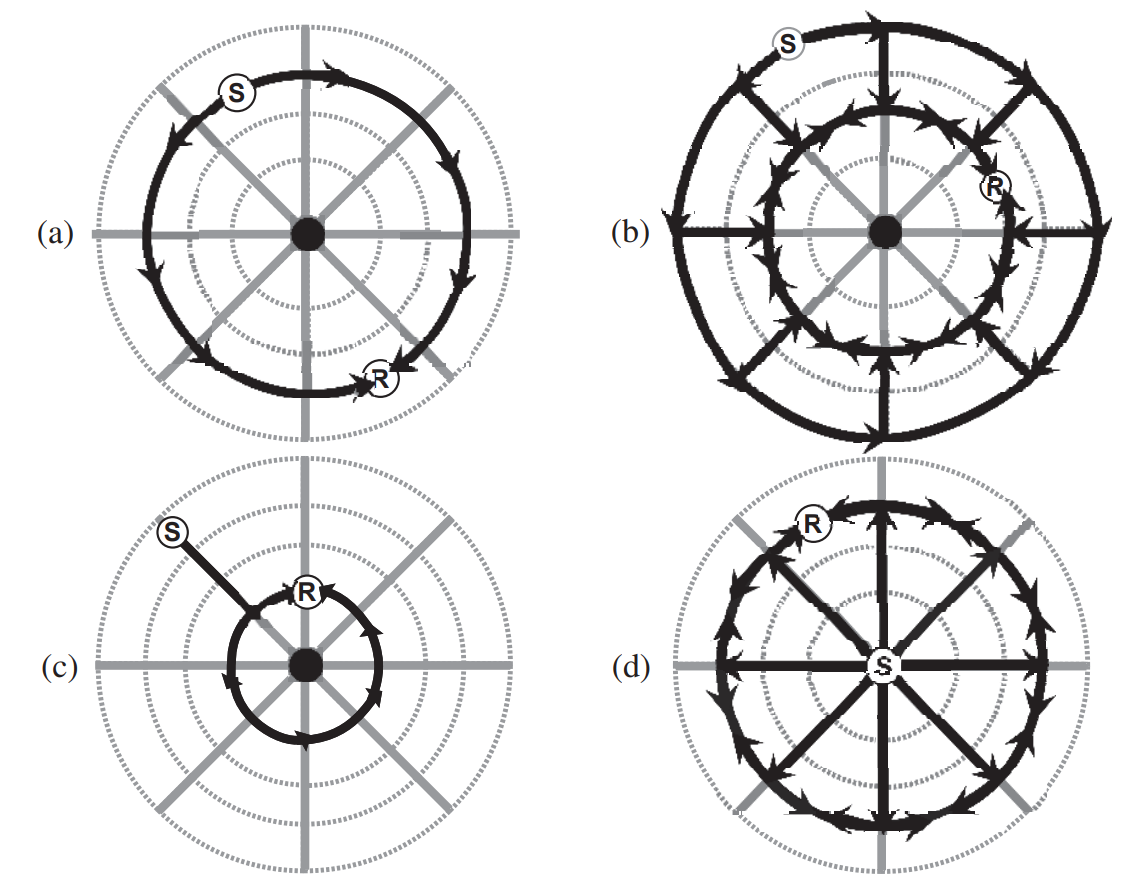
\includegraphics[width=0.75\textwidth]{images/Derous.png}
    \caption[DEROUS Protokoll Szenarien]{Darstellung von vier (a-d) verschiedenen Routing Szenarien nach dem DEROUS-Protokoll. Die schwarzen Pfeile stellen dabei die Wege dar, die ein verschicktes Paket zwischen Sender S und Empfänger R nehmen kann. \cite{liaskos2015sdm}}
    \label{fig:derous}
\end{figure}

Im Vergleich zu CORONA und anderen Routing-Systemen auf Nanoebene schneidet DEROUS gut ab. Es verringert die Anzahl von wiederholten Übertragungen und hat eine hohe Rate erfolgreicher Peer-to-Peer Übertragungen. Auch schneidet es im Vergleich zu anderen Protokollen gut ab, wenn es um die Flutungsrate geht. Dabei geht es darum, wie viel im Durchschnitt geflutet wird. Diese Rate ist in DEROUS abhängig davon, wo der Beacon gesetzt ist, jedoch sind auch worst case Szenarien noch besser als einige andere Ansätze.

Zusammenfassend lässt sich sagen, dass DEROUS einen vielversprechendes Ansatz für ad-hoc Nanonetzwerke bietet. Dabei ist es sowohl für Low-Power-Anwendungen als auch für Anwendungen mit höherem Energiebedarf geeignet. Obwohl die Betrachtung von DEROUS, ähnlich wie bei CORONA, momentan auf den zweidimensionalen Raum beschränkt ist, kann DEROUS mit relativ geringem Aufwand auf einen dreidimensionalen Raum erweitert werden. In diesem Fall würde die Kommunikation nicht radial oder kreisförmig, sondern sphärisch ablaufen.

Aus allen drei vorgestellten Arbeiten lässt sich ableiten, dass Kommunikationsprotokolle für DNA-basierten Nanonetzwerken in keiner Arbeit konkret betrachtet werden. Die meisten Arbeiten für Nanonetzwerke konzentrieren sich auf andere Materialien oder Mechanismen. Diese können als Inspiration für DNA-Tiles verwendet werden, jedoch lässt sich wegen der Eigenschaften der benutzen Materialien keines der Routing Protokolle komplett auf Nanonetzwerke mit DNA-basierter Self-Assembly übersetzen.
Nach der Betrachtung der verwandten Arbeiten und den zuvor gelegten Grundlagen kann im Folgenden das Konzept vorgestellt werden.
